Dado el siguiente escenario:

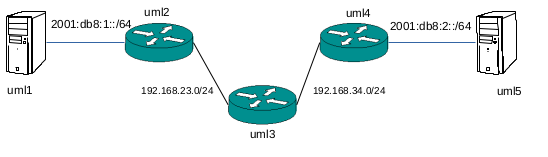
\includegraphics[width=\textwidth]{tuneles6in4}

\begin{minted}{bash}
  # net.conf
  defsw br12 uml1.0 uml2.0
  defsw br23 uml2.1 uml3.0
  defsw br34 uml3.1 uml4.0
  defsw br23 uml4.1 uml5.0
\end{minted}

\begin{minted}{lexer.py:IOSLexer -x}
  ! UML1 y UML5
  configure terminal
  int eth0
  no shutdown
  end
  write
\end{minted}

\begin{minted}{lexer.py:IOSLexer -x}
 ! UML2
 configure terminal
 int eth0
 ipv6 address 2001:db8:1::1/64
 ipv6 nd prefix 2001:db8:1::/64 ! Para que anuncie su prefijo a UML1
 no ipv6 nd suppress-ra
 quit
 int eth1
 ip address 192.168.23.1/24
 quit
 ip route 0.0.0.0/0 192.168.23.2
 ipv6 forwarding
 ip forwarding
 end
 write
\end{minted}

\begin{minted}{lexer.py:IOSLexer -x}
 ! UML3
 configure terminal
 int eth0
 ip address 192.168.23.2/24
 quit
 int eth1
 ip address 192.168.34.2/24
 quit
 ip forwarding
 ip route 192.168.23.0/24 192.168.34.2
 ip route 192.168.34.0/24 192.168.23.2
 end
 write
\end{minted}

\begin{minted}{lexer.py:IOSLexer -x}
 ! UML4
 configure terminal
 int eth0
 ip address 192.168.34.1/24
 quit
 int eth1
 ipv6 address 2001:db8:2::1/64
 ipv6 nd prefix 2001:db8:2::/64 ! Para que anuncie su prefijo a UML5
 no ipv6 nd suppress-ra
 quit
 ip route 0.0.0.0/0 192.168.34.2
 ipv6 forwarding
 ip forwarding
 end
 write
\end{minted}

\begin{minted}{bash}
 # UML2 (bash)
 ip tunnel add tunnel1 mode sit remote 192.168.34.1
 ip link set dev tunnel1 up mtu 1400
 ip route add 2001:db8:2::/64 dev tunnel1
\end{minted}

\begin{minted}{bash}
 # UML4 (bash)
 ip tunnel add tunnel2 mode sit remote 192.168.23.1
 ip link set dev tunnel2 up mtu 1400
 ip route add 2001:db8:1::/64 dev tunnel2
\end{minted}

\begin{minted}{lexer.py:IOSLexer -x}
 # TEST
 # probar desde vtysh en UML1 y UML2 que se anunció correctamente el prefijo
 show ipv6 route
\end{minted}

\begin{minted}{bash}
 # TEST
 # Desde UML2, probar un ping a UML4 y viceversa
 ping -c 5 192.168.(34|23).1
 # Desde UML1, probar un ping6 a UML5 y viceversa
 ping6 -c 5 2001:db8:(1|2):ff:fe00:5f0
\end{minted}
